\documentclass[mathserif,handout]{beamer}
%\documentclass{beamer}
\usetheme{Warsaw}
\usecolortheme{seahorse}
\usecolortheme{orchid}
\usepackage{amsmath,verbatim}
\usepackage{listings}
\usepackage[english]{babel}
\usepackage{movie15}
\setbeamercovered{transparent}

\newcommand{\Deltap}{\ensuremath{\Delta^{\!+}}}
\newcommand{\trans}{\ensuremath{{}^\mathrm{T}}}
\newcommand{\eps}{\varepsilon}
\newcommand*{\approxdist}{\mathrel{\vcenter{\offinterlineskip
\vskip-.25ex\hbox{\hskip.55ex$\cdot$}\vskip-.25ex\hbox{$\sim$}
\vskip-.5ex\hbox{\hskip.55ex$\cdot$}}}}

% \lstMakeShortInline[language=myR]�

\lstdefinelanguage{myR}
{
   language=R,
   otherkeywords={read.table, set.seed, head},
   deletekeywords={url,codes, t, dt, Call, formula,Q, R, on,by,hat,is,
col, set,start,end,deltat,zip},
   sensitive=true,
   breaklines=true,
   morecomment=[l]{\#},
   morestring=[b]",
   morestring=[b]',
   basicstyle =\ttfamily\small,
   keywordstyle=\bfseries,
   showtabs=false,
   showstringspaces=false,
   literate= {~}{$\sim$}{2},
   numberstyle=\sffamily\scriptsize,
   stepnumber=2
 }




\title{Big Data, Cloud Computing and Statistics}
\author[Darren Wilkinson --- 28/1/2015]{\textbf{\large Darren 
Wilkinson} \\
\alert{\url{http://tinyurl.com/darrenjw}}\\
School of Mathematics \& Statistics, \\
Newcastle University, UK}
\date{Statistics Research Group Seminar\\Newcastle University\\28th January, 2015}

\begin{document}


\frame{\titlepage}

\section{Introduction}

\subsection{A changing world}

\frame{
\frametitle{The social and technological context}
\begin{itemize}
\item We live in ``interesting times" --- a time of unparalleled technological advancement
\item The pace of technological change is accelerating --- it always has, but now instead of changes happening over millennia and centuries, having relatively little impact over the time span of a working life, the world is changing substantially over a period of a few years, and beyond recognition over a career
\item There is major technological disruption occurring in almost all areas of business, industry, commerce, and the public sector
\item The Higher Education sector itself is ripe for massive technological disruption (but that is a whole different talk!)
\item Technological advancement (barely conceivable 20 years ago) has enabled the routine collection and
  analysis of huge volumes of data (this talk!)
\end{itemize}
}

\subsection{Big picture}

\frame{
\frametitle{Big picture}
\begin{itemize}
\item People realised several years ago that due to the exponential decrease in storage costs there is always (potentially) more value to be had from keeping data than savings to be gained from discarding it --- we now live in an age where almost all data on everything will be kept ``forever"
\item There are many challenges to realising the potential value in all of this data, and most of these are \alert{computational}, \alert{statistical} or both
\item Computational challenges: Capturing, storing, and processing
  huge data volumes poses \alert{scalability} challenges --- these are
  most straightforwardly addressed using \alert{cloud computing}
  approaches
\item Statistical challenges: Deriving useful information and making
  informed decisions using \alert{big data}...
\end{itemize}
}

\section{Big data}

\subsection{What is it?}

\frame{
\frametitle{What is big data?}
\begin{itemize}
\item Bigger than ``normal" data, but no agreed definition
\item Data Volume
  \begin{itemize}
  \item Won't fit in RAM? Exceeds 20\% of RAM? Won't fit on a regular HDD? Won't fit in a standard relational database? Requires distributed analysis? Requires analysis in a single pass?
  \item Different ways to be ``big": many data points (large $n$), many variables (large $p$), high frequency (small $\Delta t$), data complexity (not just a data table), ...
  \end{itemize}
\item Not just about volume --- 3 V's: \alert{Volume}, \alert{Velocity}, \alert{Variety}
  \begin{itemize}
  \item Velocity: on-line analysis of large amounts of streaming data
  \item Variety: Modelling, analysing and synthesising multiple disparate sources of data in a unified way to draw conclusions not apparent from separate analyses
  \end{itemize}
\item Not just \alert{more}, but \alert{different}...
\end{itemize}
}

\frame{
\frametitle{Is big data new?}
\begin{itemize}
\item Not really --- back in 1994 (20 years ago), Walmart had 7~billion transactions
\item Term ``Big data" not really used before 2011, so what has changed?
  \begin{itemize}
  \item \alert{Ubiquity}. Automated data capture, opening up of existing data, simulations and synthetic data, exponential growth in data storage, massive increase in network bandwidth, the internet, the Internet of Things (IoT), ...
  \item Gradual realisation of latent value tied up in data --- \alert{data is not knowledge} --- very possible to be data rich but information poor
  \end{itemize}
\item Is ``big data" a passing fad?! The term itself may well be, but the subject and its implications for the future of statistical research are not. Statistics has changed irrevocably and we would be unwise to ignore this...
\end{itemize}
}

\frame{
\frametitle{Where is big data?}
\begin{itemize}
\item Business, Industry and Commerce: every company is an internet company --- every company relies on good (big) data
\item Science and Research
  \begin{itemize}
  \item Social science: social media platforms are huge data sources providing amazing insights into peoples lives and social interactions
  \item Geoscience: Data revolution due to technological advances, including cheap storage, networking, and sensors --- data integration and analysis a massive bottleneck
  \item Biology: Modern genomics generates massive complex data requiring sophisticated analysis. New sequencing technologies are currently revolutionising bioscience research
  \item Astronomy: eg. Square kilometre array (SKA) --- will be generating 1,000 exobytes per day by 2020. 
  \end{itemize}
\end{itemize}
}

\subsection{Opportunities and challenges}

\frame{
\frametitle{Big data opportunities}
Two quite different classes:
\begin{itemize}
\item \alert{Data manipulation}
  \begin{itemize}
  \item Sorting, selecting, matching, aggregating, ...
  \item eg. finding stuff (directions, shops, products, out-of-print books, ...)
  \end{itemize}
  \item Traditional concern of computer science
  \item Relatively little requirement for statistics...
\end{itemize}
}


\frame{
\frametitle{Big data opportunities}
\begin{itemize}
\item \alert{Inference}
  \begin{itemize}
  \item Predicting, forecasting, generalising, estimating underlying truth, counterfactuals, ...
  \item eg. forecasting demand for product next month, predicting other products a customer may like, identifying disease-causing genes, using survey results to understand preferences of a larger population, ...
  \item Arguably deeper conceptual challenges: eg. everything is ``significant" with enough data, requires mathematical and/or statistical modelling and abstraction, inferential frameworks, computationally intensive statistical model-fitting procedures, understanding bias, multiple testing issues, ...
  \end{itemize}
\end{itemize}
Often require a combination of the two (eg. real-time transaction fraud detection requires fast algorithms and sophisticated statistical models)
}

\frame{
\frametitle{Models and modelling}
\begin{itemize}
\item ``All models are wrong, but some are useful" --- George Box
\item ``All models are wrong, and increasingly we can do without them" --- Peter Norvig (Google)
\item Except that Norvig didn't say this!!!
\item What Norvig meant (and actually said!) was that data-driven models can often (but not always) replace theory-driven models in big data scenarios
\item Models need to be wrong in the right way...
\end{itemize}
}

\frame{
\frametitle{Models and modelling}
Two different approaches to mathematical and statistical modelling:
  \begin{itemize}
  \item Data-driven models: Top-down modelling of statistical variations in the data. Traditional statistical approach. Great for prediction, but don't give much insight, and vulnerable to over-fitting.
  \item Theory-driven models: Bottom-up modelling of generative mechanisms. More powerful, give greater insight and estimation of underlying truth, but very dangerous if theory is wrong and model mechanisms are inconsistent with data.
  \end{itemize}
Not always a sharp distinction between the two, and both approaches are (and will continue to be) valuable, but big data will perhaps lead to a bit of a swing back in the direction of data-driven models
}

\frame{
\frametitle{Big data issues}
\begin{itemize}
\item Large data sets are often collected opportunistically, and not for the purpose of answering the question that you are now interested in
\item Long-term longitudinal data sets are often difficult to exploit, as definitions, categorisations and data collection protocols often change over time
\item Multiple-testing and spurious correlations are a constant hazard
\item Selection bias issues are often obscure yet important --- and different for different data sources (eg. speed cameras and magazine surveys)
\item Privacy, confidentiality and ethical considerations affect all personal data
\end{itemize}
}

\frame{
\frametitle{Statistical challenges}
\begin{itemize}
\item \alert{Design}: Can the data being recorded actually answer the
  questions of interest? If not, can logging be modified so that it
  can?
\item \alert{Statistical data analysis}:
  \begin{itemize}
  \item \alert{Modelling}: Complex hierarchical models, time series modelling,
    event time data, network/graph data, ``data integration''
  \item \alert{Scalable inference}: Computational challenges addressed using
    \alert{conditional independence} to allow \alert{local
      computation}. Storage challenges addressed using notions of
    \alert{sufficiency} --- summarising data without information
    loss. \alert{Exchangeability} assumptions leading to both
    conditional independence and sufficiency.
  \end{itemize}
\item \alert{Decision making}: How to automate actions on the basis of
  (streaming) data: when to flag \alert{anomalies}, controlling
  \alert{false discovery rate}, decision making based on
  \alert{utility} theory
\end{itemize}
}

\frame{
\frametitle{Machine learning}
\begin{itemize}
\item Statisticians are not the only people who think that they can make sense of (big) data
\item Large and growing \alert{Machine Learning} (ML) community that is becoming increasingly sophisticated (and statistical)
\item The ML community has always had a more computational focus, and has been addressing the challenges of large and complex data sets for many years
\item The ML community is very quick to pick up on any new, powerful ideas developed by the statistical community and incorporate them into their arsenal of tools and techniques (pMCMC is a good recent example)
\item \alert{Deep learning} is showing impressive results on several different challenging problems in prediction and classification --- significantly better than the best ``statistical" models
\end{itemize}
}

\section{Cloud computing}

\subsection{Introduction}

\frame{
\frametitle{Cloud computing}
\begin{itemize}
\item Cloud computing is about doing data storage and computation ``remotely", on machines in a data centre that communicate with the outside world via the internet
\item The services provided by the data centre are to some extent generic --- it is your responsibility to make sure that they are configured to your requirements
\item You are responsible for the software, but someone else is responsible for the hardware
\item Pricing models charge for usage rather than access --- moving CapEx to OpEx 
\end{itemize}
}

\frame{ 
\frametitle{Essential cluster architecture}
\centerline{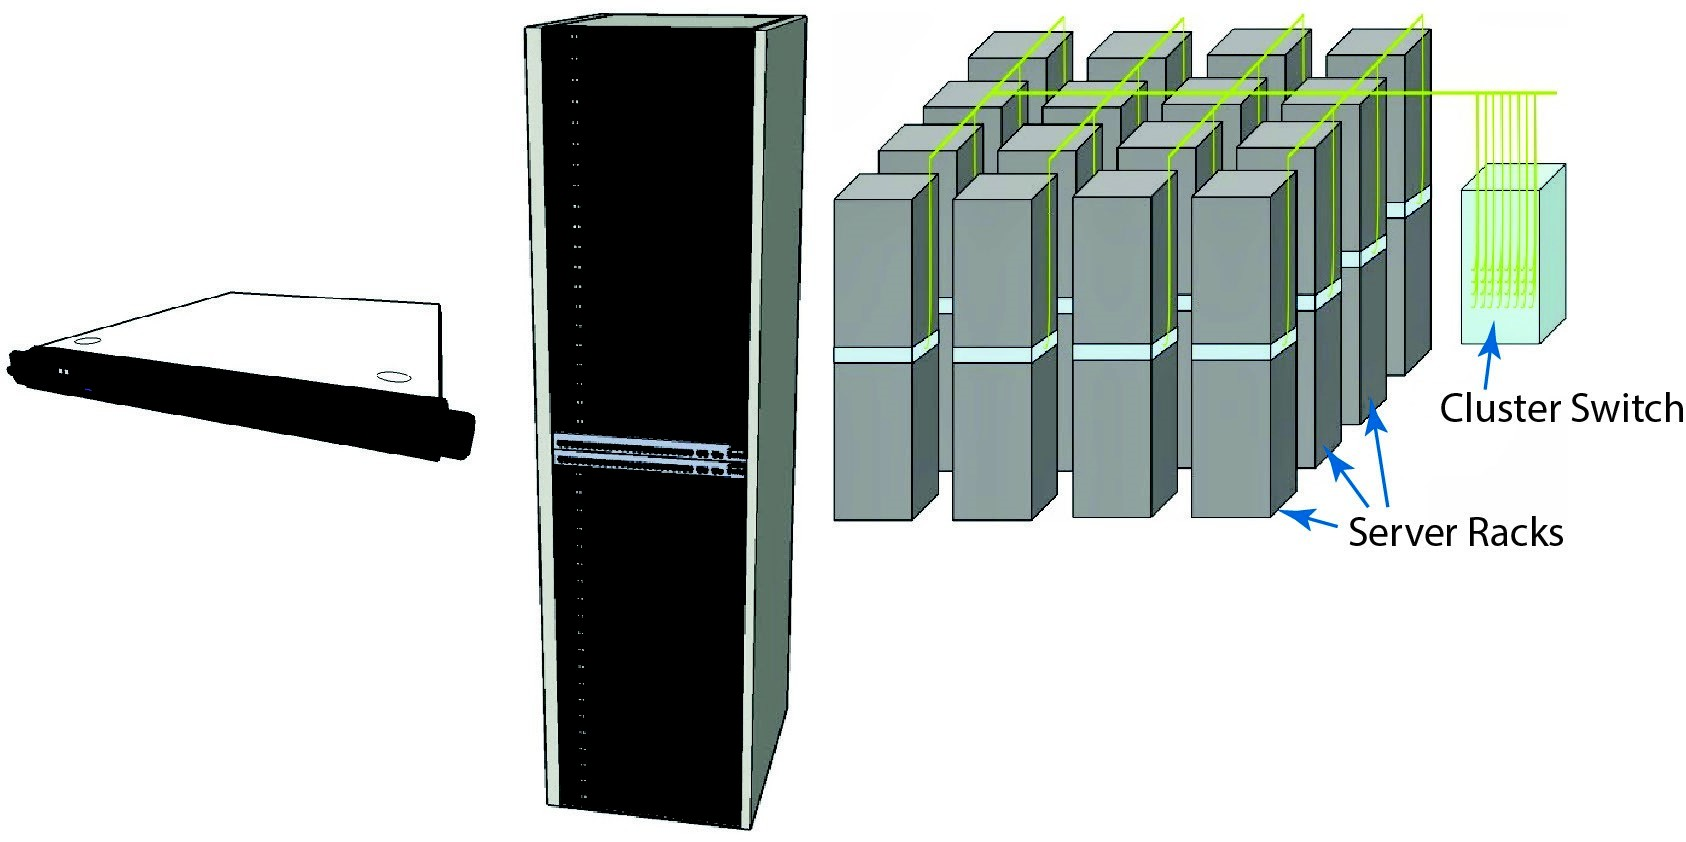
\includegraphics[width=\textwidth]{ccii-015}}
}

\frame{ 
\frametitle{A ``traditional" data centre}
\centerline{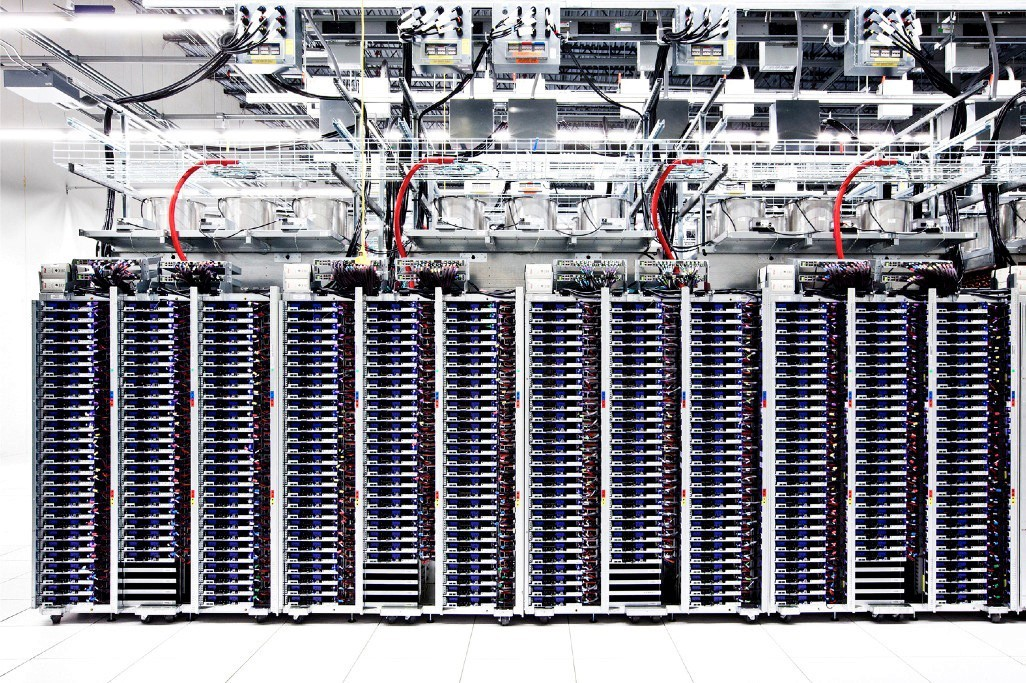
\includegraphics[height=0.8\textheight]{ccii-016}}
}

\frame{ 
\frametitle{A data centre from above}
\centerline{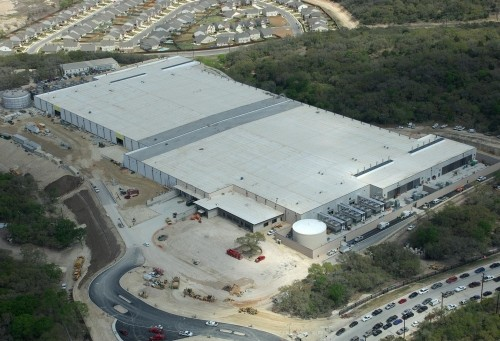
\includegraphics[height=0.8\textheight]{ccii-011}}
} 

\frame{ 
\frametitle{Inside the data centre}
\centerline{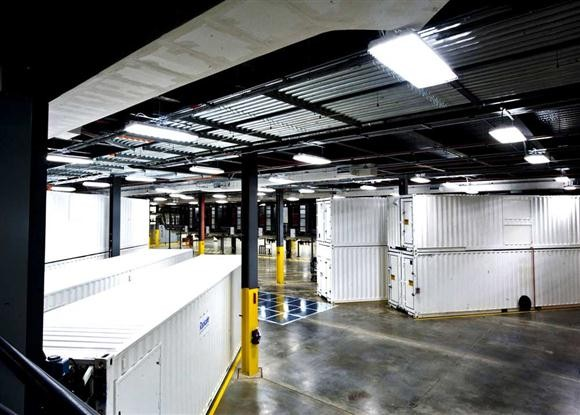
\includegraphics[height=0.8\textheight]{ccii-012}}
}

\frame{ 
\frametitle{Inside a shipping container}
\centerline{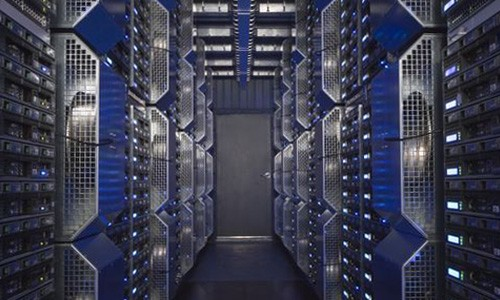
\includegraphics[height=0.8\textheight]{ccii-014}}
All about efficiency, expertise, and economies of scale
}

\subsection{Cloud computing technology}

\frame{
\frametitle{Scaling computing power}
\begin{itemize}
\item Vertical
  \begin{itemize}
  \item High Performance Computing (HPC)
  \item Fast processors, lots of RAM, high bandwidth, low-latency interconnect
  \item Hard to continue to scale-up vertically...
  \end{itemize}
\item Horizontal
  \begin{itemize}
  \item Distributed, cloud computing approach
  \item Combine the power of many low--medium power computers
  \item Need to be able to split the workload into many parallel tasks that communicate infrequently
  \item Illusion of \alert{infinite} computing resources \alert{on demand}, with no up-front CapEx --- leads to \alert{agility} and \alert{scalability}
  \item Can choose spec of required resource and pay accordingly
  \end{itemize}
\end{itemize}
}

\frame{
\frametitle{Virtual machines (VMs)}
\begin{itemize}
\item Clouds use virtual machines to share their hardware servers among a set of users
\item Each VM runs an OS and applications specific for a user
\item Each physical machine may run many VMs concurrently
\item A \alert{hypervisor} is the software layer sitting between the physical hardware and the VMs
  \begin{itemize}
  \item presents a virtualised view of the hardware to each VM
  \item each VM is completely isolated from other VMs running on the same physical hardware
  \item users can create and run VMs on cloud infrastructure --- requesting a specific OS and/or application stack
  \item virtualised data storage handled similarly
\item New technologies such as \alert{docker} provide light-weight virtualised containers, giving isolation from other VMs, yet running on the same underlying OS kernel --- faster to spin up and less wasteful of computational resources
 \end{itemize}
\end{itemize}
}

\frame{
\frametitle{Storage and data}
\begin{itemize}
\item VMs will always have some (traditional) disk-based file system storage, but this isn't always appropriate for big data
\item Simple solutions will start from large traditional file systems or relational database management systems (RDBMS) queried via SQL
\item Big data solutions (such as Hadoop) will offer distributed file systems (such as HDFS) for improved data locality (data partitioning), and/or unconventional (nosql) scalable database solutions such as SimpleDB, Cassandra, MongoDB, Neo4j, etc.
\item These platforms allow safe and efficient management of large volumes of data, sensibly partitioned for scalable data processing
\end{itemize}
}

\frame{
\frametitle{*--as--a--Service}
\begin{itemize}
\item Infrastructure (\alert{IaaS})
  \begin{itemize}
  \item eg. Amazon EC2 (Elastic Compute Cloud) --- basic VM providing OS of choice, processor/cores required and local disk
  \end{itemize}
\item Platform (\alert{PaaS})
  \begin{itemize}
  \item eg. EMR (Elastic Map Reduce), SimpleDB, ...
  \end{itemize}
\item Software (\alert{SaaS})
  \begin{itemize}
  \item eg. a full CMS, workflow manager, or application stack
  \end{itemize}
\end{itemize}
Big data applications are often developed at the PaaS level --- software such as \alert{Hadoop} provides a \alert{MapReduce} programming model for distributed computation --- this is a very simple example of a standard \alert{functional programming} (FP) design pattern...
}

\subsection{Distributed computation and functional programming}

\frame{
\frametitle{Functional approaches to concurrency and parallelisation}
\begin{itemize}
\item Functional languages emphasise immutable state and referentially transparent functions
\item \alert{Immutable state}, and \alert{referentially transparent} (\alert{side-effect} free) declarative workflow patterns are widely used for systems which really need to scale (leads to naturally parallel code)
\item \alert{Shared mutable state} is the enemy of concurrency and parallelism (synchronisation, locks, waits, deadlocks, race conditions, ...) --- by avoiding \alert{mutable state}, code becomes easy to parallelise 
\item The recent resurgence of functional programming and FP languages is partly driven by the realisation that FP provides a natural way to develop algorithms which can exploit multi-core parallel and distributed architectures, and efficiently scale
\end{itemize}
}

\begin{comment}

\frame{
\frametitle{Category theory}
Dummies guide:
\begin{itemize}
\item A ``collection" (or parametrised ``container" type) together with a ``map" function (defined in a sensible way) represents a \alert{functor}
\item If the collection additionally supports a (sensible) ``apply" operation, it is an \alert{applicative}
\item If the collection additionally supports a (sensible) ``flattening" operation, it is a \alert{monad} (required for composition)
\item For a ``reduce" operation on a collection to parallelise cleanly, the type of the collection together with the reduction operation must define a \alert{monoid} (must be an \alert{associative} operation, so that reductions can proceed in multiple threads in parallel)
\end{itemize}
}

\end{comment}

\frame{
\frametitle{Scala}
\begin{itemize}
\item The name Scala derives from ``Scalable Language"
\item It is a hybrid object-oriented/functional language
\item It supports both functional and imperative styles of programming, but functional style is idiomatic
\item It is statically typed and compiled --- compiling to Java bytecode to run on the JVM
\item It was originally developed by Martin Odersky, one of the original authors of the Java compiler, \texttt{javac} as well as Java generics, introduced in Java 5.
\item Development driven by perceived shortcomings of the Java programming language
\end{itemize}
}

\frame{
\frametitle{Scala usage}
\begin{itemize}
\item Scala is widely used in many large high-profile companies and organisations --- it is now a mainstream general purpose language
\item Many large high-traffic websites are built with Scala (eg. Twitter, Foursquare, LinkedIn, Coursera, The Guardian, etc.) 
\item Scala is widely used as a Data Science and Big Data platform due to its speed, robustness, concurrency, parallelism and general scalability (in addition to seamless Java interoperability)
\item Scala programmers are being actively recruited by many high profile data science teams
\end{itemize}
}

\begin{comment}

\frame{
\frametitle{Static versus dynamic typing, compiled versus interpreted}
%\small
\begin{itemize}
\item It is fun to quickly throw together a few functions in a scripting language without worrying about declaring the types of anything
\item But for any code you want to keep or share with others you end up adding lots of boilerplate argument checking code that would be much cleaner, simpler and faster in a statically typed language
\item Scala has a strong type system offering a high degree of compile-time checking, making it a safe and efficient language
\item By maximising the work done by the compiler at build time you minimise the overheads at runtime
\item Coupled with type inference, statically typed code is actually more concise than dynamic code
\end{itemize}
}

\end{comment}

\frame{
\frametitle{Scala ecosystem}
{\small\begin{itemize}
\item \alert{Akka} --- actor-based concurrency framework (inspired by Erlang)
\item \alert{Spark} --- scalable analytics library, including some ML (from Berkeley AMP Lab)
\item \alert{Algebird} --- abstract algebra (monoid) support library (from Twitter)
\item \alert{Scalding} --- cascading workflow library (from Twitter)
\item \alert{Storm} --- streaming analytics library (from Twitter)
\item \alert{Scalaz} --- category theory types (functors, monads, etc.)
\item \alert{Breeze} --- scientific and numerical library (including non-uniform random number generation and numerical linear algebra)
\item \alert{Saddle}/\alert{Scala-datatable}/\alert{Framian} --- data libraries (data frames, etc.)
\end{itemize}}
Large ecosystem of software libraries and developers using Scala in the big data space...
}

\section{Applications}

\subsection{Big data in my research}

\frame{
\frametitle{Big data in my research}
\begin{itemize}
\item Yeast robotic genetics (Conor, et al)
  \begin{itemize}
  \item Each experiment generates around 100K high-res images corresponding to around 50M growth measurements (0.5M time series)
  \end{itemize}
\item High-throughput sequencing (+ metagenomics) (Conor, +)
  \begin{itemize}
  \item Each experiment generates over 100M ``reads", each around 100 bp --- over 10B bp --- and that's ``old" tech...
  \end{itemize}
\item Social media (Twitter) data analysis (Rasiah)
  \begin{itemize}
  \item Over 1M geo-tagged tweets in NE England over a 3 month period (can get from the UO)
  \end{itemize}
\item Server log analytics (Rui)
  \begin{itemize}
  \item RedHat/JBoss want to be able to do sophisticated time series analysis on high frequency streaming diagnostic indicators from many servers, simultaneously, on-line, in real time...
  \end{itemize}
\end{itemize}
}


\subsection{CDT group projects}

\frame{
\frametitle{CDT Group projects}
Four group projects, for weeks 5--12:
\begin{itemize}
\item Self-quantification --- movement lab sensor data --- accelerometers, etc.
\item Urban observatory (UO) --- temperature sensor data
\item Pig pen monitoring sensor data (pig data!)
\item Indoor location sensor data
\end{itemize}
Have chosen to base all of the group projects this year around time series data from sensors --- some common ground for sharing ideas and techniques --- links nicely with the IoT
}

\subsection{The Urban Observatory (UO)}

\frame{
\frametitle{The Urban Observatory (UO)}
\begin{itemize}
\item The Urban Observatory is collecting and managing data from across Newcastle, integrating sensor platforms with citizen based data collection, geospatial and satellite data
\item It includes a new framework for integrating data into workflows, models and other applications
\item The Urban Observatory provides a baseline for gaining a richer understanding of how the city operates, and in the process repurpose and reuse the data across many different disciplines and applications
\item Demonstrator \alert{\href{http://ceg-research.ncl.ac.uk/uo/dashboard/}{City dashboard}} 
%\item It is a key part of the �50m investment by Newcastle University in Science Central
\end{itemize}
The platform is open and queryable over the internet (REST API with JSON output). For our twitter data analysis project, I just queried the 1 million most recent geo-tagged tweets from North-East England direct from the UO API
}

\frame{
\frametitle{Open data}
\begin{itemize}
\item The UO is part of a general trend towards \alert{open data}
\item UK data gradually opening up: \alert{\url{http://data.gov.uk/}}
\item Many businesses and organisations also have free APIs (eg. \alert{twitter}) or data available for free download (eg. \alert{wikipedia})
\item Also possible to ``scrape" data from the web for new uses. eg. \alert{\url{http://www.gdeltproject.org/}}
\item In science, open sharing of data is increasingly expected: eg. in bioscience, huge volumes of data archived and available for free download from organisations such as the \alert{EBI} 
\end{itemize}
}

\subsection{Conclusions}

\frame{
\frametitle{Summary and conclusions}
\begin{itemize}
\item We live in the Age of (Big) Data
\item There are great opportunities for Statisticians, so long as we are prepared to keep pace with technology and engage
\item The CDT students are trained in modern statistical computing, machine learning, cloud computing and analytics technologies --- they are well-prepared to meet the challenges of modern data science
\item There are plenty of people around the University and in local businesses with interesting and challenging big data problems that they would like help addressing
\end{itemize}
}

\frame{ 
\frametitle{Go forth and analyse...}
\centerline{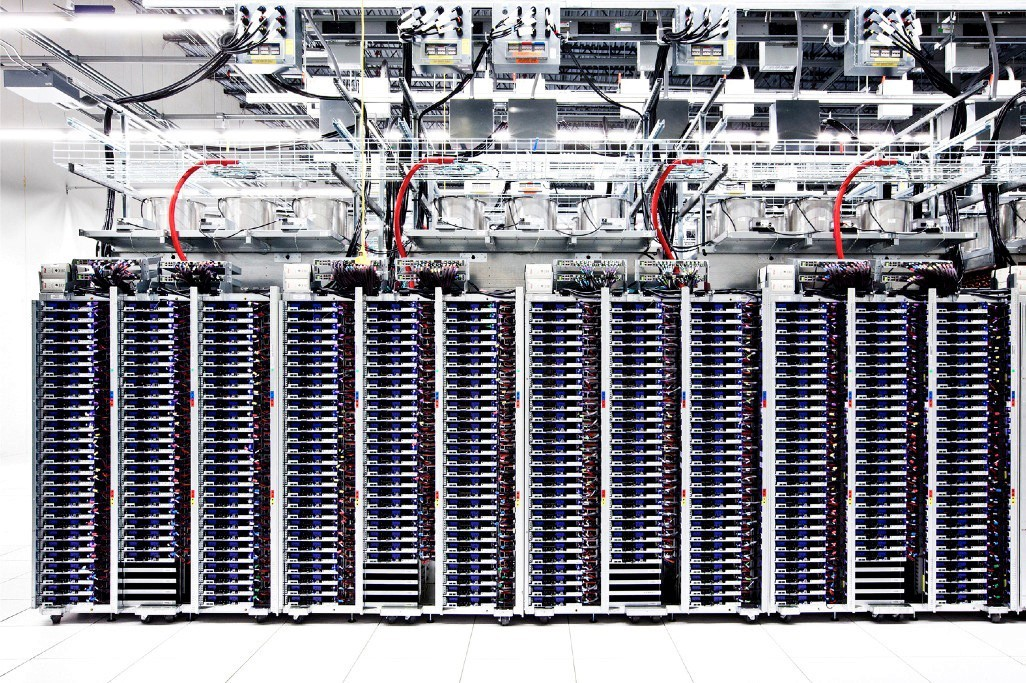
\includegraphics[height=0.8\textheight]{ccii-016}}
}



\end{document}

% eof


